\chapter{Interacciones con el blanco}

Esta clase tiene como objetivo familiarizarse con la interpretación visual de imágenes SAR. Para ello se estudiarán las interacciones con los distintos blancos para las bandas X, C y L.

\section{Interpretación visual}

En las microondas se suele hablar de tres grupos de interacciones: doble rebote, en volumen y especular, las cuales dependerán del blanco y la banda del satélite (Figura \ref{fig:interacciones}).

\subsection{Banda-X}

Abra la imagen
\begin{center}
\directory{raster\_data/CSKS1\_SCS\_B\_S2\_04\_HH\_RA\_FF\_20090321.dim}
\end{center}
correspondiente al satélite \emph{Cosmo-SKYMED}. Despliege la banda \texttt{Sigma\_HH\_db}.

Identifique en ella

\begin{enumerate}
    \item La pista de aterrizaje de la ciudad de Ushuaia.
    \item Zonas urbanas en la ciudad de Ushuaia.
    \item Zonas con vegetación sobre la ladera de la montaña.
    \item La bahía encerrada con coordenadas $54^\circ 48^\prime 51^{\prime\prime}$ latitud sur y $68^\circ 18^\prime 58^{\prime\prime}$ longitud oeste.
    \item El canal de Beagle.
\end{enumerate}

Puede ayudarse utilizando la imagen óptica.

\begin{figure}[h!]
    \centering
    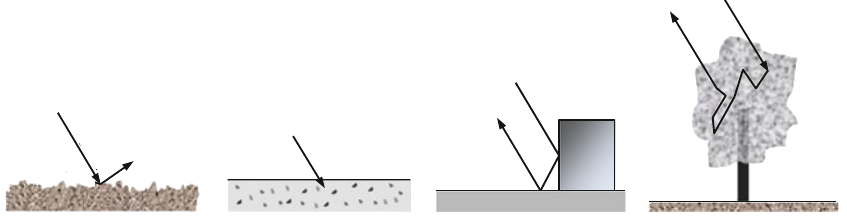
\includegraphics[width=0.9\textwidth]{fig:interacciones.png}
    \caption{Interacciónes con distintos blancos: -a- superficial, -b- subsuperficial, -c- doble rebote y -d- en volumen.}
    \label{fig:interacciones}
\end{figure}


\subsection{Banda C}

Abra la imagen
\begin{center}
  \directory{raster\_data/S1B\_IW\_SLC\_\_1SDV\_20171012.dim}
  \end{center}

correspondiente al satélite \emph{Sentinel 1B}. Despliege la banda \texttt{Sigma\_VV\_db}.

Identifique en ella

\begin{enumerate}
    \item La pista de aterrizaje de la ciudad de Ushuaia.
    \item Zonas urbanas en la ciudad de Ushuaia.
    \item Zonas con vegetación sobre la ladera de la montaña.
    \item La bahía encerrada con coordenadas $54^\circ 48^\prime 51^{\prime\prime}$ latitud sur y $68^\circ 18^\prime 58^{\prime\prime}$ longitud oeste.
    \item El canal de Beagle.
\end{enumerate}

Puede ayudarse utilizando la imagen óptica.

\subsection{Banda L}

Abra la imagen
\begin{center}
  \directory{raster\_data/ALOS-H1\_1\_\_A-ORBIT\_\_ALPSRP054716060.dim}
\end{center}
correspondiente al satélite \emph{ALOS-PALSAR 1}. Despliege la banda \texttt{Sigma\_HH\_db}.

Identifique en ella

\begin{enumerate}
    \item La pista de aterrizaje de la ciudad de Ushuaia.
    \item Zonas urbanas en la ciudad de Ushuaia.
    \item Zonas con vegetación sobre la ladera de la montaña.
    \item La bahía encerrada con coordenadas $54^\circ 48^\prime 51^{\prime\prime}$ latitud sur y $68^\circ 18^\prime 58^{\prime\prime}$ longitud oeste.
    \item El canal de Beagle.
\end{enumerate}

Puede ayudarse utilizando la imagen óptica.


\section{Valores de $dB$}

Es habitual expresar el valor del coeficiente de backscatter en dB para las imágenes SAR. Para calcularlo en distintos sectores de la imagen, puede posicionarse sobre un píxel y observar en \menu{Pixel info} el valor de \texttt{Sigma0\_HH\_db} o \texttt{Sigma0\_VV\_db} en dB.


Utilice la imagen óptica para identificar en la imagen \emph{Sentinel-1B}:

 \begin{enumerate}
     \item El valor de dB de la pista de aterrizaje.
     \item El valor de dB de las zonas urbanas.
     \item El valor de dB de las zonas con vegetación.
     \item El valor de dB para el agua de la bahía encerrada.
     \item El valor de dB para el agua del canal.
 \end{enumerate}

Se puede calcular el valor promedio de dB seleccionando una región especifica en la imagen (Apéndice \ref{ap:HA}).

Repita este análisis para las imágenes en banda X y L.

\section{Preguntas para debate}

Comparando las tres imágenes SAR utilizadas responda:

\begin{que}
    ¿Qué coberturas tienen siempre valores altos de brillo? ¿Cómo se puede interpretar la interacción?
\end{que}

\begin{que}
    ¿Qué coberturas tienen siempre valores bajos de brillo? ¿Como se puede interpretar la interacción?
\end{que}

\begin{que}
  ¿Que sucede con la vegetación sobre la ladera de la montaña al observar las imágenes en banda X, C y L?
\end{que}

\begin{que}
  ¿A que tipo de interacción corresponde cada uno de los blancos estudiados durante esta clase? ¿Depende de la imagen utilizada?
\end{que}

Estas preguntas no serán evaluadas. Su objetivo es discutirlas en el foro de sonsultas e intercambio de la clase.
